% STOA @ PVLDB Volume 20 (VLDB 2027), research track, Experiment, Analysis & Benchmark (EA&B).
% Guidelines verified 2026-10-20 (vldb.org/2027/submission-guidelines.html):
%   deadline 1st of each month 5 PM PT; abstract mandatory by the 25th of the previous month
%   single-blind (names and affiliations on page 1) | 12 pages EXCLUDING references only:
%   appendices and acknowledgements count | EA&B title suffix "[Experiment, Analysis & Benchmark]"
%   in the paper and the CMT title (dropped at camera-ready)
%   EA&B: "required to make available all experimental data and related software (there are no
%   excuses)"; the initial submission links the full reproducibility package
% Template: the official VLDB-Template bundle (github.com/vldbproceedings/VLDB-Template, commit
%   39c95f5), acmart.cls v2.19 + pvldb.sty, vendored here byte-identical to upstream.
% Build: pdflatex main && bibtex main && pdflatex main && pdflatex main
% The ICDE-formatted version is preserved as main_icde.tex; earlier PVLDB and CIDR versions as
% main_pvldb.tex and main_cidr.tex (git tag pvldb-final-2026-09).
\documentclass[sigconf, nonacm]{acmart}

%%% do not modify the following VLDB block %%
%%% VLDB block start %%%
\usepackage{pvldb}% VLDB/PVLDB formatting overrides, see pvldb.sty for details.
%%% VLDB block end %%%

\renewcommand\vldbdoi{XX.XX/XXX.XX}
\renewcommand\vldbpages{XXX-XXX}
% The reproducibility package. check_paper_numbers.py reads this macro, rejects a placeholder,
% and with STOA_CHECK_URL=1 fetches it with no credentials.
\renewcommand\vldbavailabilityurl{https://github.com/suanlab/stoa}
\newcommand\artifacturl{\vldbavailabilityurl}   % the sections cite the package by this name

\let\Bbbk\relax        % acmart's newtxmath already defines \Bbbk
\usepackage{amssymb}
\usepackage{makecell}
\usepackage{multirow}
\usepackage{cleveref}
\graphicspath{{figs/}}

\begin{document}

\title[The Unseen Block: What Split-Instant Evaluation Hides in KV-Cache Placement]{The Unseen
Block: What Split-Instant Evaluation Hides in KV-Cache Placement [Experiment, Analysis \& Benchmark]}

% Single-blind: names and affiliations are required. check_paper_numbers.py refuses the
% placeholder "STOA Project" -- the git user name that sat here unnoticed through every earlier
% PVLDB pass -- so this cannot ship unfilled.
\author{Suan Lee}
\orcid{0000-0002-3047-1167}
\affiliation{%
  \institution{Semyung University}
  \city{Jecheon}
  \country{Republic of Korea}}
\email{suanlee@semyung.ac.kr}

\begin{abstract}
A natural way to evaluate how a memory system for LLM agents should place KV-cache blocks across
storage tiers, and the one we used for three revisions of this work, is at a split instant: observe a
prefix, place the blocks that exist, and bill the result against a hindsight oracle. On two production
Mooncake traces this protocol measures little. Of the oracle's advantage, 84.4\% and 87.6\% sits on
blocks that do not yet exist at the split, so the best possible split-time policy reaches 15.6\% and
12.4\% of it; the share stays at 75--97\% for every split from 0.3 to 0.7 and under tenfold changes to
the latency and token weights, though on short traces much more is reachable. Inside that protocol a
better ranker helps monotonically, but only over that sliver. In a static analysis, deciding at each
block's arrival puts more within reach, but how much turns on a decision a split-time evaluation never
meets: where a block never seen ranks against blocks seen once. The prefix says above them (a new
block's expected reuse is 0.52 against 0.30), and ranking it there captures 2.3--4.9 times what a
clairvoyant split-time policy can; ranking it behind them can leave arrival-time placement at that
ceiling. Billed on the same metric, plain recency does better: a multi-tier LRU, which ranks every
accessed block first, captures 84.5\% and 87.7\% when moving blocks is free, and once a move costs one
read and one write none of the policies we replay that move blocks beats the static frequency heuristic. What split-instant
evaluation hides is recency and the price of migration, not a better predictor. Reactive tiering is consistent with this: LRU, LFU and a fill-once cache
reach 75--99\% (toolagent) and 40--94\% (conversation) of Belady's hit rate, the best adaptive policy (ARC, LeCaR, CACHEUS) beats
the best of those rules, each chosen per operating point, by at most 4.6 points, and a learned
replacement policy (LRB) stays below ARC, because 76--78\% of blocks are never reused. We give a one-line
diagnostic for the protocol failure, release an artifact that regenerates every number on CPU, and
catalogue the measurement defects we made and caught, including leaks in our own arrival-time experiment
that survived every number check.
\end{abstract}

\maketitle

%%% do not modify the following VLDB block %%
%%% VLDB block start %%%
\vldbtopmatter
%%% VLDB block end %%%

\section{Introduction}
\label{sec:intro}

Large language model (LLM) agents increasingly depend on memory that outlives a single context
window---the facts they extract, the turns they have seen, the tools they have run, the summaries they
have written. How well an agent answers, how fast it responds, and how much it costs are all decided by
one question asked of every memory item: \textbf{in what form should it be kept, where should it live,
and when should it be (re)materialized?} Concretely, each item can be stored as plaintext, a vector, a
graph, a latent/KV activation, or baked into parameters; it can sit on GPU, CPU, disk, or a remote tier;
and it can be written inline while serving, consolidated during an idle window, or left untouched.

Today this single decision is \textbf{fragmented across three research communities}, each of which
optimizes one axis and freezes the others. Memory-operating-system work---MemOS~\cite{F1_li2025memos},
MemGPT~\cite{P14_packer2023memgpt}---provides the primitives to migrate an item between representations
and tiers, but \emph{decides when to migrate by hand-tuned heuristics}. Reinforcement-learned memory
managers---Memory-R1~\cite{F6_yan2025memoryr1}, Memory-as-Action~\cite{F7_zhang2025memoryasaction}---learn
\emph{what content} to add, update, or delete, but operate over a single fixed representation and never
choose a tier or schedule an offline write. Systems-level cache tiering---LMCache~\cite{F5_liu2025lmcache}%
---places bytes across GPU/CPU/disk/remote to minimize \emph{miss rate or time-to-first-token}, with no
notion of the downstream task utility that the memory actually serves.

Our central observation is that \textbf{these three axes are coupled and cannot be optimized separately.}
Promoting an item to a latent or parameter representation is an expensive offline write, but it is then
cheap and fast to serve; leaving it as plaintext on disk is cheap to write but slow to read and heavy on
context tokens. The best representation depends on the tier and on how often the item will be reused; the
best tier depends on the representation's serving cost and the item's size; and whether to pay the
promotion cost at all depends on the budget. This is precisely a \textbf{budget-constrained scheduling
problem}---and a large body of ML-for-systems work (Belady-oracle imitation for cache
replacement~\cite{S2_liu2020parrot}, GNN schedulers for clusters~\cite{S5_mao2019decima}, offline-RL cache
eviction in production~\cite{S4_coldrl2025}) demonstrates that such problems are learnable.

The reason to act now is that every substrate exists but nothing orchestrates them: MemCube migration, RL
memory managers, tiered KV caches, latent memory~\cite{F2_wang2025mplus}, and sleep-time
consolidation~\cite{F3_lin2025sleeptime} all landed by late 2025, unconnected. What is missing is a
\emph{learned scheduler} that, per item and under a shared budget, trades accuracy against latency and
cost, with \textbf{task utility---not miss rate---as the objective.}

We frame this as \textbf{STOA} (Storage \& Tiered Orchestration for Agents): one budget-constrained
Markov decision process over \textbf{representation $\times$ tier $\times$ timing}, per memory item, which a
learned control plane \emph{would} solve with a serve-time latency/cost/token budget $(L,C,B)$ as its knob.
We do not build or evaluate that policy. We take the question the frame invites, \emph{is this decision
learnable?}, to production KV traces, and the measurement turned out to hinge less on the model than on
what the evaluation protocol lets a policy see: a block that does not exist yet.

A natural way to evaluate this decision, and the one earlier versions of this paper used, fixes a split
instant: observe a prefix, build features from it, place every block, and bill the result against the
future. Feature
construction can only describe a block that has been seen --- and on these traces 45--46\% of blocks have
no pre-split access at all, while the hindsight oracle they are scored against ranks them anyway. Those
blocks carry \textbf{84--88\% of the oracle's advantage}. A policy confined to the remainder looks flat
however well it ranks, which is precisely what our earlier ``ranking does not convert into placement''
result measured. We retract it.

Moving the decision to each block's \emph{arrival}, placing it the moment it first appears from the
session context available at that instant, changes what is within reach in a static analysis, but only
if one decision is made well: where a block never seen ranks against blocks already seen. The prefix says
a newly arrived block will be reused more than a block seen once; ranking it there captures 2.3 to 4.9
times what a clairvoyant split-time policy reaches (\textbf{15.6\%} and \textbf{12.4\%} of the oracle's
advantage, or 20.4\% and 15.3\% when only the tier is chosen), while ranking it behind seen-once blocks
moves arrival-time placement down by 14 to 29 points and, with tier-only actions, to that ceiling. How new blocks
are ranked among themselves moves the result by at most 5.3 points. But plain recency, billed on the same
metric, does better: a multi-tier LRU captures 84.5\% and 87.7\% when moving blocks is free, and once a
move costs one read and one write none of the policies we replay that move blocks beats the static frequency heuristic. What
the split-instant protocol hides, then, is recency and the price of migration, not a better predictor. A
synthetic control does not follow this pattern.

Reaction is competitive for a related reason. Tiering rules that forecast nothing at all --- LRU, LFU and
a fill-once cache --- reach 75--99\% of Belady's hit rate on one Mooncake trace and 40--94\% on the other,
and the whole adaptive-replacement family (ARC, LeCaR, CACHEUS) beats the best of them by \emph{at most
4.6 points}. All of them adapt on a ghost hit, and 76--78\% of blocks here are never reused, so most
evictions are correct and emit no signal: ARC gets one on 3.5--7.3\% of misses. A population of
singletons starves the channel adaptive replacement runs on.

We report how much measurement discipline this took, because it is the part most likely to transfer, and
because it is not a flattering story. Three claims were retracted, the last two only under an
adversarial review we ran with AI reviewer agents, \emph{after} the error catalogue below had been
written: a headline that randomized sampling
showed had never been measurable, the decoupling result above, and an LRB column that turned out to
measure random eviction because a training buffer was truncated to its tail. Later still, after every
number check passed, an audit of our own arrival-time experiment found that its training labels, its
split and its belief magnitudes all used information a deployed policy would not have; correcting them
withdrew four readings this paper used to make, and a later re-verification found that its order
comparison had been a magnitude comparison, withdrawing two more. In every case
the aggregate looked reasonable, which is the point --- none of our checks asked whether a reported
quantity was arithmetically able to be what it claimed, and none asked whether a stored result was
older than the program that wrote it.

\paragraph{Contributions}
\begin{itemize}
  \item \textbf{(C1)} A frame, not an evaluated system: agent-memory placement as one budget-constrained
  MDP over representation $\times$ tier $\times$ timing with a serve-time $(L,C,B)$ knob
  (\Cref{sec:formulation}), and a control-plane sketch for it (\Cref{sec:arch}). The traces carry signal
  for the tier axis only; the simulator also chooses representation and timing from placeholder cost
  tables, so we report the arrival-time result with and without those choices, offer the formulation
  as the frame the measurements are read against, and do not claim to have evaluated it.
  \item \textbf{(C2)} A timing result on production traces. A split-instant evaluation protocol
  makes 84--88\% of a hindsight oracle's advantage unreachable, because 45--46\% of blocks do not exist
  yet when it decides (\Cref{sec:reachable}); inside it, a better ranker helps monotonically but over a
  12--16\% sliver (\Cref{sec:capacity}). Deciding at each block's \emph{arrival} captures 2.3--4.9 times
  the matching split-time ceiling when unseen blocks are ranked above seen-once blocks, as the prefix
  says they should be (\Cref{sec:arrival}); on the same metric plain recency captures more when
  migration is free, and with migration priced none of the moving policies we replay beats the static heuristic.
  \item \textbf{(C3)} Measurements of reactive tiering on both sources against the adaptive-replacement
  family (ARC, LeCaR, CACHEUS) and a reimplemented LRB --- the best of them beating the best plain rule by
  at most 4.6 points of Belady across eight operating points --- together with an eviction-signal inversion
  that makes a policy tuned on one source a poor default for the other, and a measured explanation: KV
  traces are dominated by one-time blocks, which starve the ghost-hit channel the three adaptive
  policies run on and leave most of LRB's training labels censored
  (\Cref{sec:reaction}).
  \item \textbf{(C4)} A reusable evaluation protocol: twenty-seven measurement defects that each manufactured
  a plausible result here, grouped into nine mechanisms, and the cheap controls that catch them ---
  including the rule that a null is reportable only alongside the sample size that would have resolved
  it, and the rule that every edge of the source $\rightarrow$ artifact $\rightarrow$ figure
  $\rightarrow$ paper chain needs its own freshness check (\Cref{sec:protocol}).
\end{itemize}

We position STOA against prior work along the three axes it unifies in \Cref{tab:positioning}; no prior
system occupies their intersection---deciding representation, tier, \emph{and} timing, learned, under a
shared budget, with task utility as the objective.

% Positioning matrix. \checkmark = learned/decided; $\circ$ = fixed/heuristic; -- = not applicable.
\begin{table}[t]
  \centering
  \small
  \setlength{\tabcolsep}{4pt}
  \begin{tabular}{@{}lcccccc@{}}
    \toprule
    System & Repr. & Tier & Timing & \makecell{Task\\util.} & \makecell{Budget\\cond.} & \makecell{Joint\\credit} \\
    \midrule
    MemOS~\cite{F1_li2025memos}            & $\circ$ & $\circ$ & $\circ$ & $\circ$ & $\circ$ & -- \\
    Memory-R1~\cite{F6_yan2025memoryr1}    & -- & -- & \checkmark & \checkmark & $\circ$ & $\circ$ \\
    Mem-as-Act.~\cite{F7_zhang2025memoryasaction} & -- & -- & \checkmark & \checkmark & $\circ$ & \checkmark$^\dagger$ \\
    LMCache~\cite{F5_liu2025lmcache}       & -- & \checkmark & $\circ$ & $\circ$ & $\circ$ & -- \\
    Cold-RL~\cite{S4_coldrl2025}           & -- & \checkmark & -- & $\circ$ & $\circ$ & \checkmark$^\dagger$ \\
    Sleep-time~\cite{F3_lin2025sleeptime}  & -- & -- & \checkmark & \checkmark & $\circ$ & -- \\
    \textbf{STOA (proposed)}               & $\ast$ & $\ast$ & $\ast$ & $\ast$ & $\ast$ & $\ast$ \\
    \bottomrule
  \end{tabular}
  \caption{No prior system decides representation, tier, \emph{and} timing jointly---learned, under a
  shared budget, with task utility as the objective. \checkmark: learned; $\circ$: fixed/heuristic; --:
  not applicable. $\dagger$: credit for one axis only (content or eviction). \textbf{$\ast$: proposed in
  \Cref{sec:formulation}--\ref{sec:arch} and \emph{not evaluated in this paper}} --- the row states an
  intended design, not a measured capability, and \Cref{sec:evidence} gives reasons to doubt parts of it.}
  \label{tab:positioning}
\end{table}


\paragraph{Artifact} Every result in this paper is regenerated on CPU, without a paid API, by the
released package at \url{\artifacturl}; \texttt{make verify} re-derives each one from its stored result
in a few minutes, and \texttt{make reproduce-full} regenerates those results from the public traces.

\section{Motivation: Why Now}
\label{sec:motivation}

\paragraph{The substrates exist; the orchestration does not}
By late 2025 every mechanism STOA needs had been built---in isolation. MemOS~\cite{F1_li2025memos}
exposes a MemCube abstraction with primitives to migrate an item between plaintext, activation, and
parameter forms. LMCache~\cite{F5_liu2025lmcache} tiers KV-cache bytes across GPU, CPU, and remote
storage. M+~\cite{F2_wang2025mplus} maintains a latent memory with a co-trained retriever, and sleep-time
compute~\cite{F3_lin2025sleeptime} shows that precomputing during idle windows cuts test-time cost by
roughly $5\times$. RL memory managers~\cite{F6_yan2025memoryr1,F7_zhang2025memoryasaction} learn what to
write and edit. What is absent is the layer that \emph{decides}, per item and under a shared budget, which
of these mechanisms to invoke and when---a scheduler whose objective is downstream task utility rather
than cache miss-rate.

\paragraph{A worked coupling example}
Consider a single fact accessed $k$ times over a session (placeholder costs from our simulator).
As \textsf{plaintext} on \textsf{CPU} it costs nothing to write but $\sim$800 tokens on every serve, so
its serving cost grows as $800k$ tokens. Promoted once to a \textsf{latent} representation it costs a
one-off consolidation but serves at $\approx$0 tokens thereafter. For a cold fact ($k{=}1$) the promotion
never pays off; for a hot fact ($k{\gg}1$) it is decisively cheaper---and the crossover depends on the
tier (which sets read latency), on the timing (paying the promotion \textsf{online} vs.\ amortizing it in
a \textsf{sleep} window), and on the residual token budget $B$. The three axes cannot be set
independently, and the right setting is data-dependent, which is why one might want to learn it.

\paragraph{Why a control plane, and why learned}
Hand-tuned migration rules (as in today's memory-OS systems) cannot track this crossover across
workloads, budgets, and backbones. But the decision is not intractable: it is a budget-constrained
scheduling problem, and adjacent problems---cache replacement~\cite{S2_liu2020parrot,S4_coldrl2025} and
cluster scheduling~\cite{S5_mao2019decima}---have repeatedly been shown learnable from traces. STOA frames
the joint representation--tier--timing decision the same way, as a control plane that would sit above
existing stores and tiers; whether it is learnable on real traces is what \Cref{sec:evidence} measures.

\section{Problem Formulation}
\label{sec:formulation}

\subsection{The per-item decision}
An agent accumulates memory items $\mathcal{M}=\{m_1,\dots,m_N\}$---facts, dialogue turns, tool results,
summaries. For each item a memory system must answer three questions that are today decided separately:
\emph{representation} $\rho\in\{\textsf{plaintext},\textsf{vector},\textsf{graph},\textsf{latent},
\textsf{parameter}\}$, the semantic form (trading fidelity, serving-token cost, write cost);
\emph{tier} $\tau\in\{\textsf{GPU},\textsf{CPU},\textsf{disk},\textsf{remote}\}$, the physical location
(trading read latency and capacity); and \emph{timing} $t\in\{\textsf{online},\textsf{sleep},\textsf{noop}\}$,
\emph{when} the placement is (re)materialized.

The central claim is that these axes are \textbf{coupled}. Promoting an item to $\textsf{latent}$ or
$\textsf{parameter}$ is an expensive offline write but then cheap and fast to serve; leaving it as
$\textsf{plaintext}$ on $\textsf{disk}$ is cheap to write but slow to read and token-heavy. The optimal
representation depends on the tier and on reuse; the optimal tier depends on the representation's size
and serving cost. No axis can be optimized in isolation.

\subsection{A budget-constrained MDP}
We cast the orchestrator as a budget-constrained MDP solved by a learned policy $\pi_\theta$.

\paragraph{State} For each candidate item $m_i$ the state $s_t^{(i)}$ concatenates: (a)~\emph{semantic}
features---embedding, recency, access frequency, a provenance/version tag, a predicted next-access time
(a Belady-style forecast); (b)~\emph{systems} features---current representation and tier, item size, and
per-tier occupancy/pressure; (c)~\emph{budget} features---residual $L$, $C$, $B$; and (d)~\emph{query}
context. Items are the nodes of a \emph{memory graph} (edges: co-access, entity links) perceived jointly.

\paragraph{Action} Each item is assigned one action $a=(\rho,\tau,t)$. The raw space has
$|\rho|\!\cdot\!|\tau|\!\cdot\!|t|=5\!\cdot\!4\!\cdot\!3=60$ combinations, but some are illegal and are
\textbf{masked}: a $\textsf{parameter}$ promotion is sleep-only (never inline $\textsf{online}$), and
$\textsf{latent}$/KV memory is meaningful only on $\textsf{GPU}$/$\textsf{CPU}$. Masking removes
$4+6=10$ combinations, leaving a fixed legal set of $|\mathcal{A}|=50$ per item. Legality is defined
once and is load-bearing: both the action enumeration and the policy's output distribution are defined
over exactly these 50 actions.

\paragraph{Transition} Executing $a$ realizes a cost tuple $(\text{lat},\text{cost},\text{tok},
\text{fresh})$ from a transition model whose cost tables are placeholders (\Cref{sec:protocol}). Timing sets the economics: a
$\textsf{sleep}$ action amortizes the one-off promotion cost off the serving path; a $\textsf{noop}$
serves the item from its current form at no write cost.

\paragraph{Objective} We maximize expected task utility subject to serve-time budgets:
\begin{equation}
\max_{\theta}\ \mathbb{E}\!\Big[\textstyle\sum_t U(a_t)\Big]
\ \ \text{s.t.}\ \ \text{Latency}\le L,\ \text{Cost}\le C,\ \text{Tokens}\le B ,
\end{equation}
where $U$ is a downstream reward (QA accuracy, or a step-level process reward) realized only when the
item is \emph{used} to answer a query---many steps after placement. We relax the constraints with learned
duals:
\begin{equation}
r_t = U - \lambda_L\,\text{lat} - \lambda_C\,\text{cost} - \lambda_B\,\text{tok} + \beta\,\text{fresh}.
\end{equation}
The operator sets $(L,C,B)$ at serving time and the policy adapts, so a \emph{single control knob} moves
the system along its accuracy--latency--cost frontier---the key operational difference from a statically
configured memory system. We do not evaluate it here.

\subsection{A factored policy over the memory graph}
A joint head over 50 actions per item, across many items, is combinatorial. We factor the policy over a
shared trunk, $\pi_\theta(a\mid s)\propto \pi_{\text{rep}}(\rho)\,\pi_{\text{tier}}(\tau)\,
\pi_{\text{time}}(t)$, and evaluate it \textbf{only over the 50 legal joint actions}: the three factor
logits are summed for each legal $a$ and softmaxed over that set. This keeps the policy factored (three
small heads) while making the induced distribution \emph{masking-exact}---it never places probability on
an illegal combination. The trunk is a graph network over the memory graph
(\Cref{sec:arch}), so co-accessed items inform one another's placement rather than being decided
independently. Whether this policy class can actually be \emph{fit} to useful accuracy is an empirical
question, not a property of the formulation; \Cref{sec:evidence} measures the decision such a policy
would make, not the policy.

\section{The STOA Control Plane}
\label{sec:arch}

STOA is sketched as a control plane above a MemOS-style store, an LMCache-style tiering layer and an
M+-style latent path. A graph network over co-access and entity links, as Decima uses one for
scheduling~\cite{S5_mao2019decima}, feeds a factored policy whose representation, tier and timing heads
are masked to the 50 legal joint actions (\Cref{sec:formulation}), with a budget-conditioned critic. Online
actions run on the serving path; offline ones (promotion to latent or parameter forms, summarizing turns
into a graph) run in idle windows~\cite{F4_fang2025lightmem,F3_lin2025sleeptime}. Training would combine
Belady-oracle imitation~\cite{S2_liu2020parrot}, process supervision with a learned
critic~\cite{F20_xiong2025raggym} and segment-level advantages over the trajectory segments memory edits
induce~\cite{F7_zhang2025memoryasaction}, offline first, in the style of production cache-eviction
RL~\cite{S4_coldrl2025}. \textbf{None of this machinery is evaluated in this paper.} \Cref{sec:evidence}
measures the decision it would make, and finds that its value turns less on a better learned ranker than
on how far to trust a block it has never seen; we leave the policy as a design.

\section{What Placement Has To Get Right}
\label{sec:evidence}

\Cref{sec:formulation} frames placement as a learnable budget-constrained MDP. This section reports what
we found when we measured that decision on production KV traces, and it is organized around a defect rather
than a result, because the defect came first and everything else follows from it: the split-instant
protocol, which we used before, makes 84--88\% of the achievable benefit unreachable, so a
policy measured inside it looks flat however well it ranks (\Cref{sec:reachable}). Moving the decision to
each block's arrival puts more of it within reach on the production traces, and where an unseen block
ranks against seen ones then matters far more than how unseen blocks are ranked (\Cref{sec:arrival}). We then report what a
better ranker buys once the metric is repaired (\Cref{sec:capacity}), where reaction stands
(\Cref{sec:reaction}), and, at length because it is the most transferable part, the protocol,
including the three claims we retracted along the way (\Cref{sec:protocol}).

\subsection{Sources and references}
\label{sec:sources}
We use \textbf{Mooncake}~\cite{qin2024mooncake}, replayed production traces from a general LLM serving
stack (conversation, 12{,}031 requests; toolagent, 23{,}608), and \textbf{kv-cache-tester}, anonymized agentic coding
conversations (200 of 739 fetched). Each request lists the hash ids of the KV blocks it touches, so a
repeated hash is a genuine reuse. Both sources record wall-clock request timestamps. Block ids in
kv-cache-tester are conversation-scoped, so we namespace them before pooling; not doing so invents
cross-conversation reuse. \Cref{tab:regimes} summarizes both sources.

Two references bound every policy, both billed on the true future: a \textbf{hindsight oracle} that ranks
and places knowing future access counts, and a \textbf{frequency heuristic} that assumes the future looks
like the observed prefix. ``Headroom'' is
$(\text{cost}_{\text{heur}} - \text{cost}_{\text{oracle}})/\text{cost}_{\text{heur}}$; ``captured'' is the
fraction of that interval a learned policy recovers. Cost combines latency, money and context tokens
with weights $\lambda_L = 0.1$ per ms, $\lambda_C = 1$ per USD and $\lambda_B = 0.0005$ per token, which
the artifact documents as illustrative unit-normalising values and has not changed since its first
commit.

\subsection{The protocol decides what is reachable}
\label{sec:reachable}
A natural way to evaluate placement is to fix a \emph{split instant}: observe the trace up to some
point, build features from that prefix, place every block, and bill the result against what the future
turns out to contain. It is what we ran in earlier versions of this paper, and it has a structural defect
that no aggregate computed inside it can reveal.

The defect is general, not particular to our setup. Whenever a workload admits new items after the split
(that is, whenever it is not a closed working set), a split-time policy has no opinion about
those items while the hindsight oracle it is scored against ranks them freely. The reported ``fraction of
headroom captured'' then divides by a quantity that is partly unreachable, and the unreachable share
grows with the arrival rate. Any study reporting that fraction without bounding it is reporting a number
whose denominator it has not characterized.

Feature construction can only describe a block that has been seen. On these traces
\textbf{45.2\% and 46.1\% of blocks have no pre-split access at all}, and a policy therefore has no
opinion about them, but the hindsight oracle it is scored against ranks them anyway, using knowledge of
a future in which they exist. A new block's first access creates it (its KV is computed), a compulsory
miss no placement can serve, so only its later accesses are billed. Even so, new blocks carry
\textbf{84.4\% and 87.6\%} of the oracle's total advantage, so most of the denominator of every
``captured headroom'' number we reported was unreachable by construction:

\begin{center}\small
\begin{tabular}{@{}lrr@{}}
\toprule
& conversation & toolagent \\
\midrule
blocks with no pre-split access & 45.2\% & 46.1\% \\
full hindsight gap & 32{,}002 & 31{,}484 \\
\textbf{reachable gap} (visible blocks only) & \textbf{4{,}996} & \textbf{3{,}900} \\
share no causal policy can reach & \textbf{84.4\%} & \textbf{87.6\%} \\
\bottomrule
\end{tabular}
\end{center}

\medskip
\noindent\textbf{It is not an artifact of where we cut, but it needs a long trace.} Sweeping the split
from 0.3 to 0.7 leaves the unreachable share at \textbf{75.0--95.7\%} on conversation and
\textbf{77.4--96.6\%} on toolagent, worse at earlier splits, where more of the trace is still to come.
Scaling $\lambda_L$ or $\lambda_B$ by 0.1 or 10 leaves it at 79.3--97.1\%. Trace length matters more:
on the first 1{,}500 requests a split-time policy can reach 38.0\% and 57.7\% of the advantage, falling
to 15.6\% and 12.4\% on the full traces. The pathology is a property of the protocol on long horizons.

\medskip
\noindent\textbf{It is a property of arrivals, not of production.} Mooncake's third released workload
is synthetic (public datasets, Poisson arrivals), and we use it as a control rather than pool it.
Only 24.6\% of its blocks are new at the midpoint, against 45--46\% on the production traces, and the
unreachable share falls with them: \textbf{54.6\%} at the midpoint and \textbf{29.4--77.9\%} across
splits. Within every one of the three traces the share rises monotonically as the split moves earlier;
across traces the level differs, production's new blocks carrying more of the oracle's advantage than
synthetic ones at a similar new-block share. Even where only 8\% of blocks are new, almost a third of
the advantage is out of reach.

\medskip
\noindent A policy confined to 12--16\% of the prize will look flat however well it ranks, and that is
what our earlier ``decoupling'' result measured. We retract it (\Cref{sec:protocol}).

\paragraph{The diagnostic is one line} Compute the oracle's advantage twice, once with clairvoyance
over every item and once restricted to the items the policy could have had an opinion about, and take the
ratio, the \emph{reachable share}; the restricted advantage is the \emph{split-time ceiling}, the most
any split-time policy can capture. If the share is far from one, the protocol is the finding. It costs a single extra placement pass, it
needs no new data, and running it on the first day would have saved us months. We ship
it as \texttt{attainable\_ceiling} in the artifact and recommend it as a standard reporting requirement
for placement and admission studies: \emph{state the reachable share alongside any captured fraction}.

\subsection{Deciding on arrival, not at a split}
\label{sec:arrival}
Most of the oracle's advantage lives in blocks that do not exist yet when a split-time policy
decides. The alternative is an earlier decision: form each block's belief \emph{when it first appears},
from context available at that instant (the shared-prefix session's age, request rate and recency, the block's
position within its request, the request's length). Nothing the policy uses reads the future. The arrival
population is exactly the blocks first seen at or after the billing split. The model is fitted on blocks
first seen before it, each labelled by its reuse within a fixed window that closes before the split.
A belief has an order and a magnitude. Three \emph{order} arms rank new blocks by arrival (earliest
highest), by a learned score, or at random, and quantile-match that rank onto one multiset, the pre-split
blocks' access counts resampled to the number of new blocks, so they differ only in which block receives
which value. Two \emph{magnitude} arms give every new block one constant, the mean or the median of that
multiset. Two conventions the evaluation must fix are varied: whether placement may also choose a
block's representation and timing, as the cost model allows, or the tier only, the one choice physically
meaningful for a KV block; and whether a new block whose belief ties a pre-split block's goes behind it
or ahead of it. Finally, a \emph{hazard} arm replaces the convention with an estimate: at a pseudo-split
halfway through the prefix it measures how often blocks born after that point are reused before the real
split, against blocks already present, by count and age. A new block's expected reuse (0.52 and 0.48)
exceeds that of a block seen once (0.30 and 0.27), so it is placed between count 2 and count 3, never on
a tie. It gives new blocks that belief (hazard new) or every block its estimate (hazard all). Beliefs
are causal; the allocation is one static capacity-constrained assignment over the window.

\begin{center}\small\setlength{\tabcolsep}{2.4pt}
\begin{tabular}{@{}llrrrrrr@{}}
\toprule
& & & & \multicolumn{2}{c}{constant} & \multicolumn{2}{c}{hazard} \\
\cmidrule(lr){5-6}\cmidrule(l){7-8}
actions, tie & & split & order arms & mean & median & new & all \\
\midrule
all, behind  & conv & 15.6 & 38.2--41.5 & 53.4 & 29.4 & 58.2 & 69.7 \\
             & tool & 12.4 & 38.9--41.5 & 61.1 & 29.7 & 61.1 & 68.8 \\
all, ahead   & conv & 15.6 & 53.1--55.3 & 53.4 & 53.4 & 58.2 & 69.7 \\
             & tool & 12.4 & 56.6--58.1 & 61.1 & 56.0 & 61.1 & 68.8 \\
tier, behind & conv & 20.4 & 14.3--19.6 & 39.2 & 0.0 & 47.0 & 56.9 \\
             & tool & 15.3 & 15.1--19.4 & 51.7 & 0.0 & 51.7 & 54.8 \\
tier, ahead  & conv & 20.4 & 38.7--42.3 & 39.2 & 39.2 & 47.0 & 56.9 \\
             & tool & 15.3 & 44.3--46.8 & 51.7 & 43.3 & 51.7 & 54.8 \\
\bottomrule
\end{tabular}
\end{center}
\noindent{\footnotesize Percent of the full hindsight gap. ``split'' is the clairvoyant split-time ceiling;
the other columns are causal arrival-time arms. Order arms: arrival, learned (AUC 0.56 and 0.61), shuffled.}

\medskip
\noindent\emph{Ranking unseen blocks above seen-once blocks is what makes arrival pay.} Under fixed
conventions the arrival arms span 0.0--61.1\% of the advantage; with tier-only actions and new blocks
behind, the order arms land at the split-time ceiling, 14.3--19.6\% against 15.3--20.4\%. The reference multiset
is itself a convention: matching new blocks onto the pre-split counts minus each block's creation access,
the scale the bill uses, puts every order arm at 0.3--1.6 times the split-time ceiling
(6.2--21.2\%). The prefix's
mean reuse and the hazard estimate both place new blocks above seen-once ones; the hazard arm, which needs
no tie rule, captures 2.3--4.9 times the matching split-time ceiling (2.3--5.6 when old blocks are
re-estimated too), 47.0--69.7\% against 12.4--20.4\%. On toolagent it coincides with the mean arm, so the
estimate's value is the direction it gives, not its precision.

\emph{Where an unseen block ranks against seen ones matters most.} Moving new blocks ahead of
equal-belief seen blocks moves the order arms by 14--29 points (one constant arm by up to 56);
ranking new blocks among themselves moves them by at most 5.3. On the production traces arrival order alone predicts reuse with AUC 0.55--0.56 only because early arrivals
have longer to be reused (2.3--2.4 times the future accesses of late ones); given every block the same
post-arrival horizon, its AUC is 0.46 and 0.48, while the learned ranker's is unchanged.

\emph{The synthetic control does not follow.} Its split-time ceiling is 45.4\% (60.2\% tier-only) and every
arrival arm, the hazard arms included, stays below it (0.0--40.6\%).

\emph{Four external traces agree only in part.} On Alibaba's Qwen serving traces~\cite{wang2025kvcachewild}
(four workloads, 16-token blocks) the split protocol leaves 80.6--97.7\% of the advantage
unreachable, and the hazard arm reaches 1.5--15.2 times the split-time ceiling with all
actions. With tier-only actions it reaches 1.9--3.9 times on three and nothing on the
fourth (thinking), where the prefix rates seen-once blocks above new ones. The direction the prefix gives is
a regularity of these workloads, not a law.

\emph{Recency already does this, and migration decides whether anything does.} Billed on the same metric
from the same starting state with tier-only actions, a multi-tier LRU that moves every accessed block to
the fastest tier captures 84.5\% and 87.7\% of the advantage when moves are free, more than any
arrival-time arm replayed online (at most 57.3\%); caching a block only on its second access captures
$-6.2$\% and $-2.8$\%. Once a move costs one read and one write, LRU falls to $-400.5$\% and
$-401.4$\%, and no arrival-time arm, the hazard arm included, beats the static frequency heuristic; the
hazard arm keeps 70\% of its static gain only if a move costs at most 7.3\% and 7.2\% of that price.
Ranking unseen blocks first is a weaker form of recency, and whether either pays is set by the price of
migration, which the static analysis cannot see.

\emph{Earlier versions of this experiment were wrong five times, and six of their readings are
withdrawn.} The first leaked: training labels counted post-split accesses (34.3\% and 46.3\% of label
mass), its train/eval cut differed from its billing split, and its magnitudes were the evaluation blocks'
true future counts. The first causal rerun gave pre-split blocks a belief of zero in the arrival arms.
The next compared a constant-mean first-come-first-served (FCFS) arm with order arms on the spread multiset, so its order comparison
was a magnitude comparison. Every version fixed one tie convention and one action space without saying
so. And every version billed a new block's creation as a read from its tier, which inflated the full
gap about three times (2.5 with tier-only actions). Withdrawn: that a learned ranker captures less than
FCFS, that FCFS captures 87\% and 50\% of what is reachable, that arrival order is worth 14 points, that
FCFS leads the ranker by 2 to 26 points, that this lead reflects exposure time, and that timing recovers
nothing on the synthetic control, which the corrected bill has since made true again.

The design implication: build an \textbf{admission point}, and \emph{estimate}, rather than assume,
where it ranks an unseen block against blocks already seen. Baleen~\cite{S12_wong2024baleen} is the one
system among those we survey that decides admission rather than eviction, and it optimizes a downstream
system cost rather than miss rate.

\subsection{What a better ranker buys inside the split protocol}
\label{sec:capacity}
Within the split-instant protocol, does a stronger model convert into a better placement? Each rung is
trained on one trace and evaluated on the other, so the AUCs are cross-trace. With ties broken by tier
speed and every belief quantile-matched onto one magnitude multiset, the scored blocks' own pre-split
counts, so that only the ordering varies:

\begin{center}\small
\begin{tabular}{@{}lrrr@{}}
\toprule
rung & AUC (conv / tool) & \% of ceiling (conv) & (tool) \\
\midrule
constant        & 0.50 / 0.50 & $-48.6$ & $-60.6$ \\
random          & 0.49 / 0.50 & $-62.7$ & $-284.0$ \\
$\log$(count)   & 0.64 / 0.71 & $0.0$   & $0.0$ \\
logistic        & 0.81 / 0.93 & $+50.7$ & $+55.0$ \\
GBDT            & 0.80 / 0.91 & $+47.6$ & $+44.9$ \\
MLP             & 0.82 / 0.93 & $+52.6$ & $+59.5$ \\
\midrule
ceiling         & 1.00        & $100$   & $100$ \\
\bottomrule
\end{tabular}
\end{center}

\medskip
\noindent Ranking quality converts monotonically on both traces. $\log$(count) reproduces the frequency
heuristic exactly, since it ranks by the same counts the magnitudes come from, and each better model
recovers more, the best about half of the split-time ceiling. But that ceiling is the 12--16\% of
\Cref{sec:reachable}: the strongest model gains 8.2\% and 7.4\% of the oracle's advantage. A previous
version of this table placed every rung on the evaluation blocks' true future counts, which no deployed
policy has; there every rung fell below the heuristic and conversion failed on one trace.

\paragraph{The magnitude convention moves the result more than ranking does}
Running each rung twice, once on the scale its own scores naturally produce and once on the common
multiset, \emph{with the ordering identical in both}, gives:

\begin{center}\small
\begin{tabular}{@{}llrrr@{}}
\toprule
trace & rung & native & common & $\Delta$ \\
\midrule
conversation & logistic & $+74.1$ & $+50.7$ & 23.4 \\
             & $\log$(count) & $-40.7$ & $0.0$ & $-40.7$ \\
             & random   & $-84.5$ & $-62.7$ & $-21.8$ \\
\midrule
toolagent    & logistic & $+87.8$ & $+55.0$ & 32.7 \\
             & $\log$(count) & $-25.2$ & $0.0$ & $-25.2$ \\
             & random   & $-665.4$ & $-284.0$ & $-381.5$ \\
\bottomrule
\end{tabular}
\end{center}
\noindent{\footnotesize Percent of the split-time ceiling. The two columns differ only in the magnitudes
attached to an identical ranking.}

\medskip
\noindent The same policy, with the same ordering, scores $+87.8\%$ or $+55.0\%$ depending on a choice of
scale, and across rungs the scale moves the result by \textbf{22 to 381 points}, more than any ranking
difference above. We report the common-scale column, where only ordering varies, and make the
methodological point: \textbf{``fraction of headroom captured'' is not a quantity until the magnitude
convention is stated}, and none of our earlier drafts stated it.


\begin{table}[t]
  \centering \small \setlength{\tabcolsep}{4pt}
  \begin{tabular}{@{}lrr@{}}
    \toprule
     & \makecell{Mooncake\\(serving)} & \makecell{kv-cache-tester\\(agentic)} \\
    \midrule
    requests analysed              & 12{,}031 / 23{,}608 & 4{,}215 (40 conv.) \\
    blocks touched exactly once    & 75.8 / 78.5\% & 15\% \\
    mean reuse per block           & 1.6 / 2.2 & 26 \\
    blocks per request             & 24 / 17 & $\sim$1{,}900 \\
    block size (tokens)            & 512    & 64 \\
    \midrule
    headroom, heuristic vs.\ oracle & 80\%  & 68--73\% \\
    \bottomrule
  \end{tabular}
  \caption{The two sources, at the scales actually analysed. Mooncake pairs are conversation /
  toolagent; its headroom averages the two (79.9\% and 79.8\%). The agentic column is the first 40
  conversation files, except headroom, which is the mean over four randomized draws of 20 and of 40
  conversations (\Cref{sec:sampling}). Its descriptive statistics are sample-dependent: the one-time
  fraction ranges 7.5--21\% over 20--200 conversations. An earlier revision took this column's headroom
  from nested-prefix samples (81--94\%), the protocol \Cref{sec:sampling} retracts.}
  \label{tab:regimes}
\end{table}


\subsection{A measurement that was never a measurement}
\label{sec:sampling}
We also attempted the obvious follow-up (fit a richer per-block model on the agentic source and place
with it) and first obtained what looked like a strong positive: $+66$ to $+88\%$ of the headroom
captured, reproducing across what we took to be two samples. It was not a result, and the way it failed is
worth more than the number would have been.

The two samples were \emph{sorted prefixes} of the conversation corpus, so the smaller was contained in
the larger; and file index correlates strongly with conversation shape (mean requests per conversation
falls from 140 to 37 between files 1--20 and 71--150). Extending the same prefix to 100 and 150
conversations drove the captured headroom to $-9\%$ and $-48\%$ --- a sign reversal. Re-drawing the
samples \emph{at random} rather than as prefixes then showed why: four random draws at 40
conversations land between $-166$ and $+66$ points, and at 20 conversations between $-858$ and $+78$
(\Cref{tab:kvct}). The spread dwarfs the effect by an order of magnitude. We quote the observed range
rather than a confidence interval on purpose: with four draws a parametric interval rests on a normality
assumption these data cannot support, and \emph{captured} is a ratio whose denominator varies per draw.
An earlier revision of this paper reported $\pm126$ here, computed with the normal quantile against a
standard deviation estimated from four points; the correct $t(3)$ half-width is $\pm166$ on the current
artifact. That error was ours. Under a correct sampling protocol there was never a
measurement here to report.

We keep this in the paper for two reasons. It is the control that our own protocol
(\Cref{sec:protocol}) lacked, and running it costs minutes; and it bounds what the rest of our numbers
are worth, since every other result in this section is also a single draw of a parameter we chose.

\begin{table}[t]
  \centering \small \setlength{\tabcolsep}{5pt}
  \begin{tabular}{@{}lcc@{}}
    \toprule
    & \makecell{sorted-prefix samples\\(as first reported)} & \makecell{4 random draws\\mean [observed range]} \\
    \midrule
    20 conversations & --- & $-541\%$ $[-1207, +78]$ \\
    40 conversations & $+88\%$ & $-67\%$ $[-234, +66]$ \\
    70 conversations & $+75\%$ & --- \\
    100 conversations & $-9\%$ & --- \\
    150 conversations & $-48\%$ & --- \\
    \bottomrule
  \end{tabular}
  \caption{Headroom captured by a learned placement policy on agentic traces, the same pipeline measured
  two ways. Left: sorted-prefix samples, which are nested and drawn from a corpus whose per-conversation
  statistics vary threefold along the file index --- the numbers we first reported (regression variant,
  all features), and their reversal; an earlier revision printed the classifier's $+87\%$ at 70.
  Right: randomized draws at the same sizes, summarized by their observed range --- four draws cannot
  support a parametric interval. The spread is an order of magnitude wider than any effect, so this
  quantity was never measurable under this protocol. We report it as a cautionary measurement.}
  \label{tab:kvct}
\end{table}


\subsection{Where reaction stands}
\label{sec:reaction}
The alternative to forecasting is to react. On the full Mooncake traces, reactive tiering
reaches 75--99\% of Belady's hit rate on the toolagent trace and 40--94\% on open-ended conversation
using LRU, LFU or a fill-once cache alone; admitting the adaptive and learned policies below widens the
per-operating-point envelope only to 76--99\% and 42--94\% (\Cref{fig:reactive}).

The interesting question is not the envelope --- that is an oracle over policies, not something anyone
deploys --- but whether any \emph{single} policy attains it, and whether the adaptive designs built for
exactly this situation beat plain rules. We therefore run the family: \textbf{ARC}~\cite{S7_megiddo2003arc},
which shifts a recency/frequency split on ghost hits; \textbf{LeCaR}~\cite{S8_vietri2018lecar} and
\textbf{CACHEUS}~\cite{S9_rodriguez2021cacheus}, which replace ARC's arithmetic update with regret-based
multiplicative weights over two experts; and the learned \textbf{LRB}, which is reported separately below because its
numbers carry an implementation band the others do not.

\begin{center}\small
\begin{tabular}{@{}lrrrrr@{}}
\toprule
trace & tier & best pure & ARC & LeCaR & CACHEUS \\
\midrule
conversation & 2\%  & 39.8 & 29.4 & \textbf{42.3} & 35.9 \\
             & 5\%  & 53.3 & \textbf{57.9} & 56.8 & 53.5 \\
             & 10\% & 76.0 & \textbf{77.5} & 77.2 & 75.3 \\
             & 20\% & \textbf{94.1} & 87.4 & 93.9 & 88.8 \\
\midrule
toolagent    & 2\%  & 74.9 & 70.7 & \textbf{75.8} & 73.9 \\
             & 5\%  & 81.3 & \textbf{83.6} & 83.0 & 82.9 \\
             & 10\% & 91.9 & 92.3 & \textbf{92.9} & 91.8 \\
             & 20\% & 99.3 & 96.3 & \textbf{99.3} & 97.6 \\
\bottomrule
\end{tabular}
\end{center}
\noindent{\footnotesize Percent of Belady's hit rate. ``Best pure'' is the better of LRU, LFU and a
fill-once cache at that operating point.}

\medskip
\noindent Across eight operating points and four designs, \textbf{the best adaptive or learned policy
beats the best pure rule by at most 4.6 points of Belady}, and at the loosest tier by at most 0.1. Which
design wins also moves: LeCaR at the tightest tier on both traces and ARC at 5\%; above that, ARC and
then plain LRU on conversation, LeCaR on toolagent. That is the substantive finding --- not that these policies fail, but that on KV-block workloads
the whole adaptive-replacement family collapses into a band a few points wide, well short of the oracle
at the small tiers where the decision actually matters.

The diagnostics say why, and the reason is specific to KV workloads. Every policy in this family adapts
on a \emph{ghost hit} (a miss on a block it recently evicted), whether it updates a split (ARC) or
an expert weight (LeCaR, CACHEUS). But 76--78\% of blocks in these traces are never reused at all, so
most evictions are correct and produce no signal. Measured, ARC receives an adaptation signal on
\textbf{3.5--7.3\% of misses}; the regret-based policies read the same channel, which is why they land
in the same band rather than above it. What signal it does get is not merely sparse but, at
the smallest tier, directionally wrong: at a 2\% tier ARC drives $p$ to 90\% recency on both traces, while
the rule that actually wins there is frequency. A workload whose blocks are mostly singletons starves the
very mechanism adaptive replacement runs on.

\paragraph{And the learned cache policy loses to both --- but only as a range} The natural learned
baseline is LRB~\cite{S6_song2020lrb}, which learns a relaxed-Belady objective from
a far richer feature set than our four trace-local statistics and won on production CDN traces. We
reimplement it: GBDT regression on log time-to-next-request over inter-access deltas and exponentially
decayed counters, sampled eviction, online retraining from a sliding memory window, right-censored
labels.

Our first version of it measured something else entirely. The training buffer was capped by truncating to
its tail; labelled rows arrive one at a time as blocks are re-accessed while censored rows arrive in one
contiguous burst per checkpoint, so from the third retrain onward every training label was identical, the
regressor returned a constant, and eviction degenerated to a uniform draw over the sampled candidates.
We report the repaired numbers and, because two defensible repairs disagree, we report them as a band:

\begin{center}\small
\begin{tabular}{@{}lrrrr@{}}
\toprule
trace & tier & LRB (repaired) & ARC & below ARC? \\
\midrule
conversation & 2\%  & 27.6--29.2 & 29.4 & yes \\
             & 5\%  & 30.9--32.2 & 57.9 & yes \\
             & 10\% & 45.0--45.9 & 77.5 & yes \\
             & 20\% & 75.8--76.5 & 87.4 & yes \\
\midrule
toolagent    & 2\%  & 68.8--69.0 & 70.7 & yes \\
             & 5\%  & 71.1--71.4 & 83.6 & yes \\
             & 10\% & 80.9--83.0 & 92.3 & yes \\
             & 20\% & 94.6--94.9 & 96.3 & yes \\
\bottomrule
\end{tabular}
\end{center}
\noindent{\footnotesize Percent of Belady. The band spans two repairs of the truncation bug: subsampling
all accumulated rows, and dropping rows older than the memory window first. We adopt the second, which is
what a ``sliding memory window'' means.}

\medskip
\noindent \textbf{What the band supports.} The two repairs agree to within 2.1 points at every operating
point, and \textbf{LRB is below ARC at all eight operating points under both.} That ordering is the claim
we make; the numbers are context for it. Both repairs and the retracted behaviour are selectable in the
artifact, so the band is regenerated rather than reported. We do not claim the band bounds every
reasonable reimplementation: a third repair produced in an AI-agent review we ran (see the Acknowledgment)
reported a higher figure, and since its code is not ours to ship, we neither reproduce nor rely on it.

The mechanism appears to be the one that limits ARC, seen from the other side. LRB learns from labels the
trace supplies when a sampled block is requested again; a block that never returns yields a
\emph{right-censored} row, which says only ``not within the window'' and nothing about when. At the
default window \textbf{83--88\% of LRB's training rows are censored}, and 88--91\% at a shorter one. A
population dominated by singletons starves the ghost-hit channel that adaptive replacement runs on and
the regression target that learned replacement runs on, for the same underlying reason.

Three caveats bound this. It is our reimplementation of the published mechanism, not the authors'
artifact. KV blocks are uniform-size, so byte miss ratio collapses to object miss ratio and LRB loses one
of its structural advantages over LRU. And the hyperparameter sweep we ran to check that the result was
not a tuning artifact was run on the \emph{broken} implementation, so it tested the robustness of random
eviction; we have not repeated it.


The eviction signal also inverts by source. On the agent traces LRU reaches 0.83--0.96 of Belady at a 5\%
tier while LFU stays near 0.29--0.31; on Mooncake the ordering reverses below the working-set knee. An
eviction policy tuned on one source is a poor default for the other --- and, as both the ARC and the LRB
result show, reaching for a more sophisticated policy does not by itself resolve the choice.

\begin{figure}[t]
  \centering
  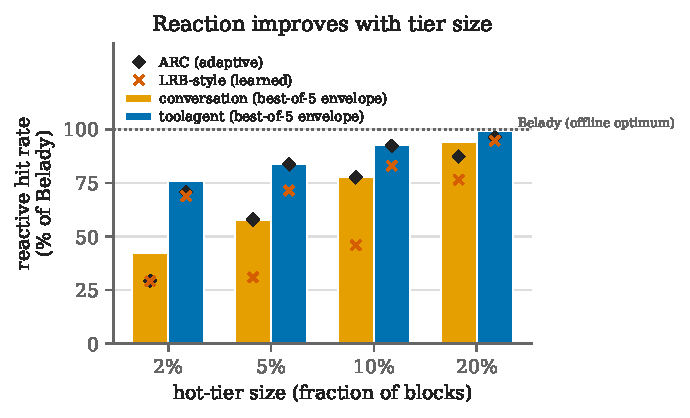
\includegraphics[width=\columnwidth]{fig_reactive.pdf}
  \caption{Reactive tiering as a fraction of Belady's hit rate, full Mooncake traces. Bars are a
  per-operating-point best-of-seven envelope, an oracle over policies rather than a policy. Diamonds are
  ARC, which meets the envelope at 5\% on both traces and at 10\% on conversation but falls short
  elsewhere; crosses are the
  LRB-style learned policy, which is below ARC everywhere.}
  \label{fig:reactive}
\end{figure}

\subsection{What the measurement required}
\label{sec:protocol}
Every positive result we obtained before the final protocol was an artifact, and each looked reasonable:
a flat captured fraction, a plausible interval, a learned policy landing below ARC. Two of the
twenty-seven defects in \Cref{tab:defects} were found by an adversarial review we ran with AI reviewer
agents (see the Acknowledgment), five by an audit and the rest by re-verification passes, all after the
paper had passed every check it defined for itself. The artifact's lab notebook records each one with
its fix.

\begin{table*}[t]
\centering\footnotesize
\begin{tabular}{@{}p{3.2cm}p{8.6cm}p{4.9cm}@{}}
\toprule
mechanism (count) & what happened & control now in the harness \\
\midrule
Reference-frame mismatch (6) & a split over access-event indices that fell past the trace's end; ties
broken by label (AUC 0.51 to 0.94); an oracle inheriting the heuristic's order; features built at one
split instant, costs billed at another & one split instant for features, labels and bill; frames compared
explicitly \\
Retracted claims (3) & retracted: a ``+66--88\% captured'' agentic headline that sampling showed was never
measurable; the \emph{decoupling} claim, an artifact of an unreachable denominator; an LRB column that
measured random eviction because its training buffer was truncated & randomized draws; the reachable
share beside any captured fraction; LRB fails on zero label variance \\
Free-parameter extrapolation (3) & curves read from one point: a cache size, a trace length, a
conversation count (+88\% reversing to $-48\%$) & every convenience parameter swept \\
Believing a report (1) & an edit script printed success after matching nothing & edits asserted to land \\
Stale derived or parallel surfaces (3) & artifacts older than the code that made them; figures fifteen
days older than their data; a notebook stating a falsified claim & content-hash provenance; figure and
PDF manifests; banners on records \\
Unchecked summaries (1) & a sentence misquoted a checked band's width & spans and maxima asserted;
withdrawn values must be absent \\
Unverified interventions (1) & a mutation whose target string was absent ``passed'' & interventions
asserted to apply; guards tested both ways \\
Emphasis without verification (1) & the headline share sat in no artifact and mixed two references
(97\% to 95\%, then 84--88\%) & every emphasised number asserted \\
Leaks and unstated conventions (8) & in the arrival experiment: post-split labels; a cut unlike the bill;
magnitudes from evaluation blocks' futures; zero beliefs for pre-split blocks; a mixed-scale ceiling; an
order control that also changed magnitude; unstated tie and action-space conventions (up to 56 points);
creations billed as reads (the gap inflated about three times) & a causal module with an AST taint test;
conventions swept; billable access defined in one place \\
\bottomrule
\end{tabular}
\caption{The twenty-seven measurement defects, by mechanism. Each produced a plausible number that matched
its artifact.}
\label{tab:defects}
\end{table*}

Two of them changed what this paper claims. A headroom taken at 1{,}500 requests moved by full length
from 86.4\% to 91.8\% on toolagent and from 82.9\% to 93.5\% on conversation, and a protocol evaluated
on short traces would have found far more reachable than the full traces show (\Cref{sec:reachable}).
And the conventions of \Cref{sec:arrival}, each fixed for convenience, moved one arm by up to 56 points.
Three controls would have caught most of the catalogue on the first day: compute the reachable share
beside any captured fraction; treat every convenience choice as a variable to sweep; and, before
reporting a null, compute the sample size that would have resolved it, because ``we could not tell'' and
``there is nothing there'' are different claims. The harness ships with these wired in, and with a
checker that re-derives every result in this paper from its artifact and fails on drift.

\subsection{Limitations}
\label{sec:limits}
No real vLLM+LMCache deployment was measured, so any cost-expressed quantity should be read as a range.
We tightened what that range means. Our first sensitivity analysis scaled every tier latency by a common
factor, which moves the absolute scale and leaves the \emph{ratios} between tiers untouched --- and the
ratios are what a placement policy responds to, so it never tested the parameter that mattered. We
therefore derive the table instead: KV bytes per block follow exactly from a model's attention shape
($2 \times \text{layers} \times \text{kv\_heads} \times \text{head\_dim} \times \text{dtype}$ per
token), and per-tier latency is that divided by a declared device-class bandwidth plus a fixed overhead.
Sweeping three attention shapes against five device classes puts headroom at \textbf{55--98\%}, which
contains the 92\% our hand-written table gives --- the headroom conclusion survives (we did not rerun the
unreachable share or the arrival arms under the derived tables), but two things about the
table do not. Its GPU:CPU latency ratio is 1:10 where every device class but the deliberately flat one gives 1:80 to 1:250, an order of
magnitude in the ratio the policy is most sensitive to; and \textbf{6 of the 15 configurations reorder
the hierarchy} so that latency order and capacity order disagree, which our fixed per-tier capacity table
cannot express at all. Calibrating against a live deployment remains the open gate; this is the honest
intermediate, not a substitute. The
\emph{timing} and \emph{representation} axes of \Cref{sec:formulation} are chosen by the simulator from
placeholder cost tables but carry no signal from the traces, which is why \Cref{sec:arrival} also reports
tier-only placement. A
representation pilot over three textual fidelities is in the artifact, but it depends on
a paid hosted model, and this paper reports only what the artifact regenerates without one. Both
sources are KV-block hash streams from transformer prefix caching, so they are independent in provenance
but not in mechanism. Alibaba's four traces (16-token blocks) and Mooncake's synthetic control broaden the
set, but we still cannot separate workload character from vendor, date, or block size. Sampling is not randomized, every placement result is
a single deterministic run, and no confidence interval is reported for them, though trace length, split
instant, cost weights, tie convention and action space are now swept rather than fixed. The arrival-time
arms form beliefs causally but are allocated capacity in one static assignment, which is neither a bound
nor an admission policy: replayed online they need nearly free migration to keep their gain (above).
The hazard estimate fixes one pseudo-split, its count bins and its age quartiles, and applies counts from
half the prefix to counts over the whole of it; rescaling for that moves the hazard arm by at most 0.6 points on the production traces. Of the learned and adaptive cache literature we evaluate
ARC~\cite{S7_megiddo2003arc}, LeCaR~\cite{S8_vietri2018lecar}, CACHEUS~\cite{S9_rodriguez2021cacheus} and
a reimplementation of LRB~\cite{S6_song2020lrb}; Hawkeye, Mockingjay and Baleen are positioned in
\Cref{sec:related} but not run, the first two because a KV block hash carries no analogue of the program
counter their predictors are indexed by. Our LRB is the
published mechanism rebuilt from the paper, not the authors' artifact (as are our LeCaR and CACHEUS, whose
CR-LFU expert we approximate by LFU), and the uniform block size of both sources removes one of LRB's
advantages over LRU, so the underperformance we report should be read as a statement about this workload
rather than about these designs.

\section{Open Problems}
\label{sec:open}

Our result closes one question and sharpens several others.

\paragraph{What should an admission point believe about a block it has never seen?}
\Cref{sec:arrival} shows that deciding at arrival puts more of the oracle's advantage within reach, and
that the result then turns on one decision: where a block never seen ranks against blocks seen once. The
prefix gives its direction; learning it per session or per request, and admitting online at a migration
cost low enough to keep the gain, which our replay did not find under a read-plus-write price, is the
obvious next model. Ranking new blocks against each other is a second-order question, and comparing rules on it needs
an evaluation that gives every block the same exposure, a rolling window or a fixed post-arrival horizon,
because in a finite trace early arrivals have more time to be reused. Whatever such an evaluation leaves
unclaimed has to come from something the per-item formulation does not express: admission under
contention, coordinated eviction across concurrently-live sessions, or migration timed against idle
windows.

\paragraph{Calibration, and what a mis-specified cost model hides}
Our tables are placeholders, and we saw concretely how misleading that is: under them the per-item optimal
action is identical for every reused block, which collapses a three-axis decision into a one-dimensional
sort and makes every policy look alike. Fitting the tables to a real vLLM+LMCache deployment --- the only
GPU-gated step in this work --- is a precondition for any claim about the representation and timing axes,
which our traces do not exercise at all.

\paragraph{Aggregate working set, not per-request footprint}
Reactive sufficiency is governed by how much of the \emph{concurrently live} working set a tier holds, not
by one request's block count: holding tier size fixed in absolute blocks and raising the number of pooled
conversations still degrades the ratio. Characterizing that surface --- tier size against concurrency,
across sources --- would give an operator a sizing rule, which is the most directly actionable thing this
line of work could produce.

\paragraph{Composing placement with retrieval}
Placement sets latency and cost; retrieval sets which facts reach the model. The open problem is the
composition --- a retriever running over a tiered store whose hot set a scheduler maintains, where a
retrieval miss on a cold tier costs latency rather than accuracy. Neither literature evaluates that
joint object, and the KV traces here cannot: they record block reuse, not which facts a query needed.

\paragraph{Sampling as a first-class experimental variable}
Three of the defects in \Cref{sec:protocol} were extrapolations from a single value of a parameter fixed for convenience, and
the most damaging reversed a headline claim's sign. For trace-driven work we would now require of
ourselves, and suggest for the area: randomized rather than prefix sampling, several disjoint draws with
intervals, and a reported sweep over every quantity the design fixes --- trace length, pool size, tier
size, split fraction --- before any claim that depends on one of them.

\paragraph{Safety and governance}
A memory written by tools and other agents is an attack surface, and provenance must survive consolidation
so a fact can be traced, invalidated, or unlearned. A budget-constrained scheduler is a natural
enforcement point; doing that without giving back the frontier is unexplored.

\section{Related Work}
\label{sec:related}

We organize prior work by the three axes STOA unifies; \Cref{tab:positioning} summarizes which axis each
line decides and by what means.

\paragraph{Representation and memory-OS.}
MemOS~\cite{F1_li2025memos} and MemGPT~\cite{P14_packer2023memgpt} treat memory as an operating-system
problem, exposing abstractions (MemCube, virtual context) and primitives to migrate items between
plaintext, activation, and parameter forms; M+~\cite{F2_wang2025mplus} adds a co-trained latent memory.
These provide the \emph{mechanism} to change representation and tier but decide \emph{when} by heuristic;
STOA supplies the learned scheduler they lack.

\paragraph{Content and RL-based management.}
Memory-R1~\cite{F6_yan2025memoryr1} and Memory-as-Action~\cite{F7_zhang2025memoryasaction} learn, with
RL, \emph{what} to add, update, or delete and how to edit context, and the latter handles the
trajectory-fracturing that edits cause. But they operate over a single fixed representation and never
choose a physical tier or schedule offline consolidation---orthogonal to, and composable with, STOA.

\paragraph{Systems tiering and ML-for-systems.}
Serving systems already make prefix KV blocks reusable: PagedAttention~\cite{kwon2023pagedattention}
manages them in pages that requests can share, SGLang~\cite{zheng2024sglang} reuses them across
requests through a prefix tree, and CachedAttention~\cite{gao2024cachedattention} and
Mooncake~\cite{qin2024mooncake} keep them across a hierarchy of storage tiers, with hand-designed
policies for what stays where; our traces come from the last of these.
LMCache~\cite{F5_liu2025lmcache} tiers KV-cache bytes to cut miss-rate; H2O~\cite{S1_zhang2023h2o} evicts
by attention score. The learnability of such decisions is established: PARROT~\cite{S2_liu2020parrot}
imitates a Belady oracle for cache replacement, Cold-RL~\cite{S4_coldrl2025} does eviction with offline
RL in production, and Decima~\cite{S5_mao2019decima} schedules clusters with a GNN policy. STOA inherits
these techniques but changes the objective from miss-rate to downstream \emph{task utility}, and the
action from a single axis to the joint representation\,$\times$\,tier\,$\times$\,timing decision.

\paragraph{Offline consolidation.}
Sleep-time compute~\cite{F3_lin2025sleeptime} and LightMem~\cite{F4_fang2025lightmem} show the value of
precomputing and consolidating memory offline, but treat it as a global mode rather than a per-item,
budget-aware timing decision---the third axis STOA learns.

\paragraph{Learned and adaptive caching.}
Two lines bear directly on our results and we position against them explicitly, because our findings
reproduce rather than extend them. \textbf{LRB}~\cite{S6_song2020lrb} learns a relaxed-Belady objective
for CDN caching from a feature vector built out of the deltas between an object's past request
times --- the same family as the session recency and rate features our arrival-time ranker uses. Timing as a
cache-scheduler input is therefore established practice; what we add is evidence about \emph{when} a
placement decision is taken, not a new signal to take it with. \textbf{ARC}~\cite{S7_megiddo2003arc} adaptively balances recency against
frequency precisely because neither dominates across workloads; the recency-versus-frequency inversion we
measure between our two sources (\Cref{sec:reaction}) is that observation restated on KV blocks, and an
adaptive policy of the ARC family is the baseline a deployment should reach for rather than either pure
rule.

The rest of the learned-cache literature divides by what it learns \emph{from} and what it decides, and
the division explains why our result is not a contradiction of it.
LeCaR~\cite{S8_vietri2018lecar} and CACHEUS~\cite{S9_rodriguez2021cacheus} learn no per-item model at all:
they run experts (LRU/LFU, and in CACHEUS scan- and churn-resistant variants) and update expert weights
from regret observed on a ghost list. That is the same evidence channel ARC uses, and
\Cref{sec:reaction} measures how thin it is here --- 3.5--7.3\% of misses carry any signal --- so the
family inherits the limitation rather than escaping it. We ran both to check, rather than leaving it as a
prediction, and both land in the same few-point band as ARC. LeCaR is nonetheless the best single policy
at the tightest tier on both traces, which is the one place the regret formulation visibly pays.
Hawkeye~\cite{S10_jain2016hawkeye} and Mockingjay~\cite{S11_shah2022mockingjay} are the closest
antecedents to what we attempted: both supervise a predictor with Belady replayed over history, Hawkeye
as a binary cache-friendly/averse label and Mockingjay as a multiclass reuse-distance estimate. They
operate at CPU last-level-cache granularity, where a program counter identifies a reuse pattern; a KV
block hash carries no analogous instruction identity, which is the structural reason their signal does
not simply port. Baleen~\cite{S12_wong2024baleen} is the one that decides admission and prefetching
rather than eviction, and the one that optimizes a downstream system cost (disk-head time) instead of
miss rate --- the closest precedent for the multi-objective reward of \Cref{sec:formulation}, and the
direction we think is right even though we do not evaluate it here.

Of these we evaluate LRB, LeCaR and CACHEUS (\Cref{sec:reaction}); Hawkeye, Mockingjay and Baleen are
positioned but not run.

In short, each line optimizes one axis and freezes the others, and none decides representation, tier,
\emph{and} timing jointly under a shared budget (\Cref{tab:positioning}). Our contribution is not a better
policy but a measurement: on production KV traces the usual split-instant protocol leaves most of a
hindsight oracle's advantage out of any policy's reach, deciding at each block's arrival brings much of
it back into reach, and we report the protocol needed to see that.

\section{Conclusion}
\label{sec:conclusion}

For every item an agent remembers, three coupled questions (in what representation, on which tier, and
when to materialize it) are today answered separately by three research communities. We offered a single
budget-constrained formulation as a frame and measured one of its axes, placement across tiers, on
production KV traces.

The finding is about when to decide, and it is first a finding about evaluation. Evaluated at a split
instant, as is natural, at least three-quarters of a hindsight oracle's advantage is out of reach of any
policy that places the blocks present at the split, for every split we tried and under tenfold changes
to the cost weights; inside that protocol a better ranker helps
monotonically, but over a sliver. Deciding at each block's arrival puts more within reach on both
production traces when a block never seen is ranked above blocks seen once, as the prefix says it should
be: 2.3--4.9 times the split-time ceiling in a static analysis, a gain that needs nearly free migration to
survive online. On a synthetic control it does not. Reactive tiering, forecasting nothing, already delivers much of the
achievable hit rate, and the adaptive-replacement family adds little to it, because the signal it adapts on
is scarce when most blocks are never reused.

We arrived here only after removing twenty-seven measurement defects, each of which had produced a
plausible result, including leaks and an unfair control in our own arrival-time experiment that were
found after every number check had passed. We report their mechanisms and the controls that catch them, because the same
traps are open to anyone measuring a memory scheduler. The next steps are an admission rule that learns the belief it gives unseen blocks, an evaluation
with equal exposure per block, a cost model calibrated against real tiers, and the habit of asking what a reported
fraction's denominator could have been.


% Counts toward PVLDB's 12 pages (only references are excluded). Written to be checkable: every
% claim about what the AI did is visible in the artifact's commit history (Co-Authored-By trailers).
\begin{acks}
\textbf{Use of AI-generated content.} An AI assistant (Anthropic's Claude, Opus~5 and Opus~5.5 models,
used through the Claude Code agentic environment) was used extensively throughout this work. It wrote
most of the code in the released artifact, designed and ran most of the experiments and analyses,
drafted and revised most of the text, and generated the figures from the stored results; its contributions are recorded commit by commit in
the artifact's history. The ``adversarial review'', the audit and the re-verification passes referred to in
\Cref{sec:protocol} were internal exercises in which AI agents were prompted to act as reviewers; none
was peer review, and one
figure the review produced (a third LRB repair) is neither reproduced nor relied on here. Every result in this paper is
re-derived from the released artifact by a checker shipped with it; a few historical figures (what an
earlier version reported) come from the artifact's lab notebook. The initial concept and research
idea were proposed by the author. The author takes full responsibility for the content of this paper.
\end{acks}

\bibliographystyle{ACM-Reference-Format}
\bibliography{../docs/references}

\end{document}
